% vim: set textwidth=78 autoindent:

\subsection{Plugin Testo delimitato}\label{label_dltext}

% when the revision of a section has been finalized, 
% comment out the following line:
%\updatedisclaimer

Il plugin Testo delimitato permette di caricare un file di testo delimitato come layer in QGIS.

\minisec{Requisiti}

Per vedere un file di testo delimitato come layer, il testo deve contenere:

\begin{enumerate}
\item Una riga capopagina delimitata di nomi di campo. Questa deve essere la prima riga del file di testo.
\item La riga capopagina deve contenere un campo X ed uno Y. Questi campi possono avere qualsiasi nome.
\item Le coordinate x e y devono essere specificate da numeri. Il sistema di coordinate non è importante.
\end{enumerate}

Come esempio di un file di testo valido importiamo il file di dati dell'elevazione di un punto \filename{elevp.csv} presente nel dataset di esempi di QGIS (Vedere la Sezione~\ref{label_sampledata}):

\begin{verbatim} 
X;Y;ELEV
-300120;7689960;13
-654360;7562040;52
1640;7512840;3
[...]
\end{verbatim}

Alcune note circa il file di testo:

\begin{enumerate}
\item Il file di testo usato come esempio usa \mbox{$;$} come delimitatore. Qualsiasi carattere può essere usato per delimitare i campi.
\item La prima riga è la riga capopagina. Essa contiene i campi X, Y e ELEV.
\item Nessun tipo di virgoletta ({\tt{}"{}}) dev'essere usata per delimitare i campi di testo.
\item Le coordinate x sono contenuto nel campo {\em X}.
\item Le coordinate y sono contenuto nel campo {\em Y}.
\end{enumerate}

\minisec{Uso del Plugin}
Per usare il plugin si deve aver QGIS in funzione ed usare il Gestore dei Plugin per caricarlo:

Avviare QGIS, quindi aprire il QGIS Plugin Manager scegliendo \mainmenuopt{Plugin} > \dropmenuopttwo{mActionShowPluginManager}{Gestione Plugins}
\index{plugin!manager}
Il gestore dei plugin mostra una lista dei plugin disponibili. Quelli già caricati hanno una crocetta nella casella alla sinistra del loro nome.
Cliccare sulla casella alla sinistra del plugin \checkbox{Aggiungi layer di testo delimitato} e premere il pulsante \button{OK} per caricarlo come descritto nella Sezione \ref{sec:managing_plugins}.

Cliccare la nuova barra degli strumenti \toolbtntwo{delimited_text}{Aggiungi layer di testo delimitato} per aprire la finestra di dialogo Aggiungi layer di testo delimitato come mostrato in Figura
\ref{fig:delim_text_plugin_dialog}.

\begin{figure}[ht]
   \begin{center}
   \caption{finestra di dialogo Aggiungi layer di testo delimitato \nixcaption}\label{fig:delim_text_plugin_dialog}\smallskip
   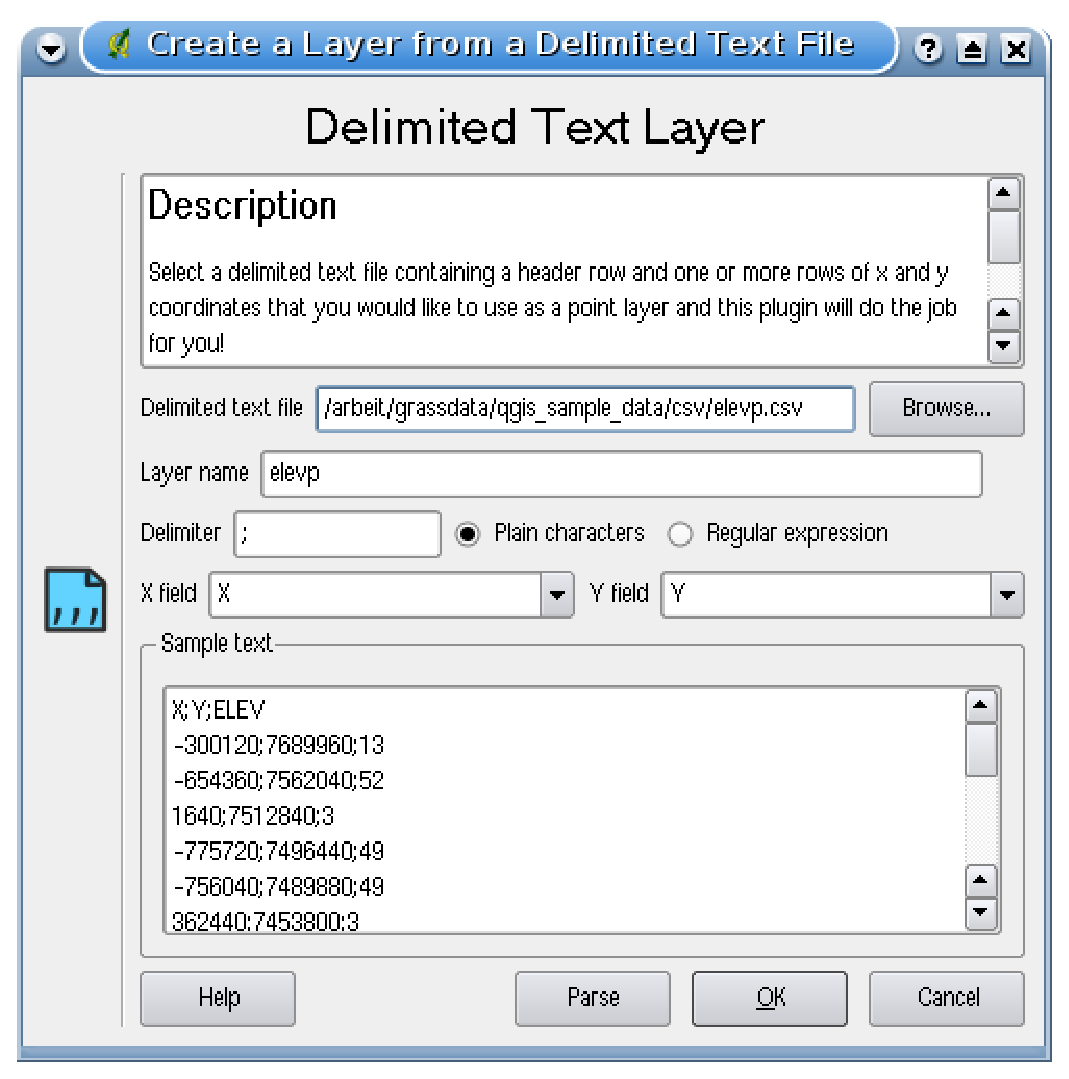
\includegraphics[clip=true, width=14cm]{delimited_text_dialog}
   \end{center}
\end{figure}

Prima selezionare il file \filename{qgis\_sample\_data/csv/elevp.csv} per importare premendo il pulsante \button{Sfoglia}. Una volta selezionato il file, il plugin cerca di processare il file usando l'ultimo delimitatore utilizzato, in questo caso \mbox{$;$}. Per processare per bene il file, è importante selezionare il giusto delimitatore. Per cambiare delimitatore a tab usare \mbox{$\backslash$}t (questa è un'espressione regolare per il carattere tab).
Dopo aver cambiato il delimitatore premere \button{Processa}.

scegliere i campi X e Y dai menu a tendina e introdurre il nome di un layer \filename{elevp} 
come mostrato in Figura \ref{fig:delim_text_plugin_dialog}. Per aggiungere il layer alla mappa, premere il pulsante \button{Aggiungi Layer}. il file di testo delimitato si comporta ora come qualsiasi altro layer di QGIS.
